\documentclass[12pt,a4paper]{article}
\usepackage{pgf-umlcd}
\usepackage[T1]{fontenc}
\usepackage[utf8]{inputenc}
\usepackage[french]{babel}
\usepackage{fullpage}
\usepackage{hyperref}
\usepackage{lmodern}
%\usepackage[colorlinks=true,breaklinks=true,linkcolor=blue]{hyperref}

\usepackage{amsmath}
\usepackage{url}
\usepackage{amsfonts}
\usepackage{amssymb}
\usepackage{listings}
\usepackage{graphicx}
\usepackage{array}
\usepackage{etoolbox}
\usepackage{xcolor}
\usepackage{listings}
\usepackage{caption}
\usepackage{makeidx}

\begin{document}
\begin{titlepage}
\begin{flushright}
      \rhead{Le \today}
\end{flushright}

\begin{figure}[ht]
  \begin{flushleft}
    
\includegraphics[width=0.5\textwidth]{./images/unicaen.png} 
  \end{flushleft}
\end{figure}


\vspace*{\stretch{1}}\parindent=0pt

\hrulefill
\begin{center}\bfseries\Huge
   Éditeur de livres dont vous êtes le héros
    	
\end{center}
\hrulefill





\begin{flushright}\bfseries\Large
\textit{\Large travail personnel approfondi}
\end{flushright}

\vspace*{2cm}


\begin{small}
 \textbf{Réalisé par:}\\
 Mahamadou Doucouré\\
Aissata Camara\\
Adama Lo\\
 Abdou Diatta\\
\end{small} 

    \vspace*{\stretch{2}}
\begin{flushright}
      L2 Informatique\\
      Groupe 4A\\
      Année 2019-2020\\
\end{flushright}   
\end{titlepage}

\newpage
\setcounter{page}{1}
\tableofcontents

\thispagestyle{empty}
\setcounter{page}{0}
%\section{Introduction}
%\section{Historique}
%\subsection{denomination}
%\subsection{mecanisme du jeu}
%\section{Organisation du projet}
\newpage
\chapter{INTRODUCTION }
\addcontentsline{toc}{part}{Introduction}
\paragraph{}Dans le cadre de notre deuxième année de Licence Informatique  à l’Université de Caen Normandie nous avons eu pour tâche la réalisation d'un projet informatique sur le module d’enseignement nommé TPA\footnote{TPA signifie «Travail Personnel Approfondi »}. 
\paragraph{}Par groupe de quatres, il nous a été demandé de réaliser des applications complètes sur différentes thèmes: CoreWar, Simulateur pour N corps, Éditeur de livres dont vous êtes le héros, etc. Parmis ces propositions si plusieurs ont retenu notre intention, une plus que, les autres, a capté notre intérêt: \textbf{Éditeur de livres dont vous êtes le héros.}   
\section{Objectifs}
\paragraph{} Pour chaque projet à réaliser, il y'a quelques objectifs à atteindre. Pour cela on nous a donner comme énoncé :
\paragraph{}«Les livres dont vous êtes le héros (ou LDVEH) sont des jeux de rôles en solitaire dont la narration est décomposées en paragraphes, dispersés dans le livre. Des liens, en fonction des choix du lecteurs, permettent d’aller d’un paragraphe à l’autre. Dans un premier temps, il s’agira de développer un éditeur de texte qui maintienne le graphe du jeu et qui puisse réorganiser aléatoirement le livre. L’affichage de la ou les solutions (paragraphe devant être traversés pour gagner) devront être calculées ainsi que la difficulté du jeu (proportions de solutions au regard des chemins possibles). Dans un second temps, il s’agira d’ajouter un système de rencontres et de combat, ainsi que la gestion d’objets ou d’indices qui peuvent être nécessaire pour gagner. Enfin, un mode lecture permettant de jouer au LDVEH pourra être implanté.» \\
On a trois objectifs à réaliser dans ce projet :\\

\begin{itemize}
	\item Le développement d'un éditeur de texte qui maintien le graphe du jeu et réorganise aléatoirement le livre. Le calcul de l'affichage des solutions ainsi que la difficulté du jeu.
	\item Ajouter un système de rencontres et de combat, ainsi que la gestion d’objets ou d’indices qui peuvent être nécessaire pour gagner.
	\item Un mode lecture permettant de jouer au LDVEH\footnote{LDVEH signifie «Livre dont vous êtes le héros »} pourra être implanté
\end{itemize}
\section{Historique}
\paragraph{}Les livres-jeux (en anglais : gamebook), souvent appelés livres dont vous êtes le héros en Francea et au Québec, sont un genre de romans ayant pour caractéristique d'être interactifs1, le déroulement de l'histoire dépendant des choix du lecteur.
\paragraph{}Ce genre, né dans les années 1960-1970, devient célèbre en 1982 avec le livre Le Sorcier de la Montagne de feu. Le genre connaît son heure de gloire dans les années 1980 et au début des années 1990 avant de sombrer dans l'oubli, les éditeurs abandonnant la réédition de ces livres dont le succès n'est plus au rendez-vous, du fait de la concurrence des jeux vidéo.
\paragraph{}Un léger renouveau se fait sentir à partir de 2003, lorsque l'éditeur anglais Wizard Books réédite les livres les plus connus de la série Défis fantastiques, suivi en 2007 par Gallimard en français. 
\paragraph{}Dans les années 2010, des éditeurs de littérature jeunesse « classique » éditent des livres-jeux en extension de leurs collections habituelles, ce qui tendrait à banaliser ce genre littéraire.\cite{ref3}\\
\section{{Fonctionnement du jeu}}
\paragraph{}Les LDVEH\footnote{LDVEH signifie «Livre dont vous êtes le héros »} sont des livres dont les paragraphes sont numérotés. À la fin de la lecture d'un paragraphe, le lecteur a le choix entre plusieurs possibilités, représentant les actions du personnage qu'il incarne. Ces possibilités renvoient à d'autres paragraphes, qui développent les conséquences des choix du lecteur. Les paragraphes ne sont donc pas lus dans l'ordre des numéros, et chaque lecteur ne lira pas les mêmes paragraphes, puisqu'il ne fera pas les mêmes choix. On peut à ce titre distinguer deux grandes familles de livres-jeux : 
\begin{itemize}
    \item Les livres « divergents » : chaque choix modifie le cours de l'histoire et mène vers une fin différente ; c'est le cas des livres des collections Choose Your Own Adventure et Le Challenge des étoiles ;
    \item Les livres « à objectif » : le personnage principal a un objectif, une mission, et les différents cheminements reviennent vers cet objectif ; il y a en général une « grande fin » qui correspond à l'accomplissement de la mission ; c'est le cas de la plupart des livres-jeux.\cite{ref2}
    
\end{itemize}
\paragraph{}Pour notre jeu on a choisi le jeu des livres à objectif.

%\usepackage{tkz-graph}
%\usetikzlibrary{arrows}


\newpage

\section{Organisation du projet}
\subsection{Répartition des tâches}
\paragraph{}Le projet étant constitué de trois objectifs nous avons décidé de faire un cahier de charge un plus détaillé. Pour cela chacun est allé faire des recherches sur la modélisation, après on a rassemblé les idées pour le faire.
\paragraph{} Ensuite il était question de réaliser les liens. Diatta et Aissata ce sont charger de schématiser le graphe\footnote{Le grapge décrit le schéma des liens c'est à dire le passage d'un paragraphe à un autre.} de notre programme. 
\paragraph{}Doucouré et Adama ce sont chargés de la réalisation l'interface graphique et son fonctionnement. Aissata et Diatta ont continué le travail du graphe tout en faisant le programme du graphe.Ensuite on  rassemblé le travail pour faire les liens à savooir sur le choix des paragraphes , les numéros de paragraphes, la suppression...
\paragraph{}Enfin on rassemblait nos idées pour le bon fonctionnement du programme.
\subsection{Architecture du programme}
    \subsubsection{Diagramme de Classe}
    \begin{figure}[ht]
  \begin{center}
    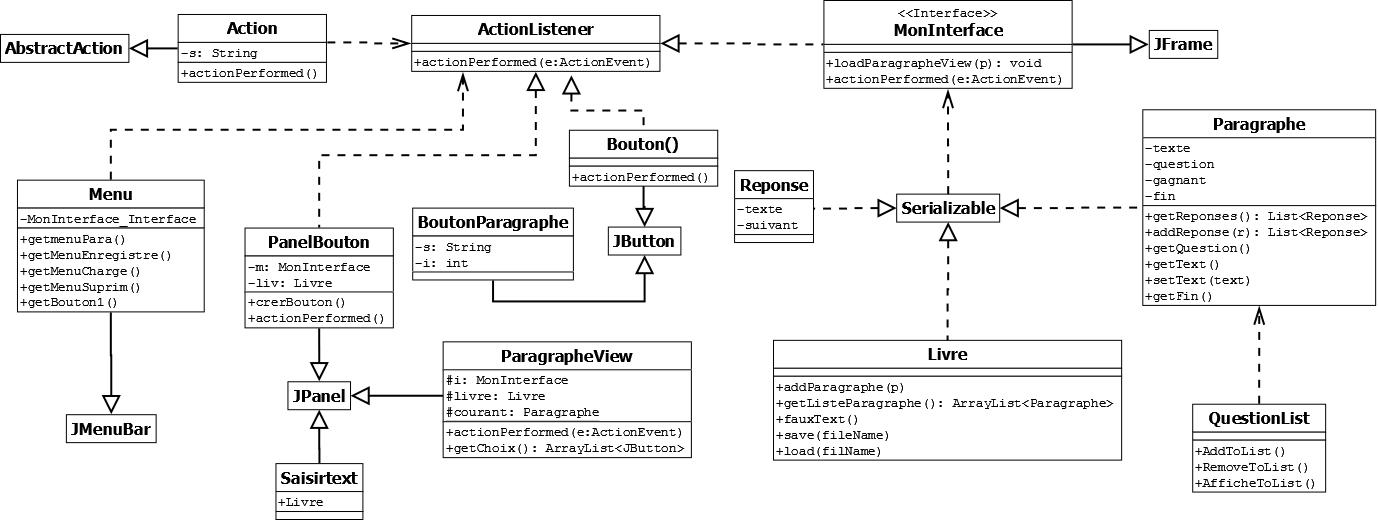
\includegraphics[width=1.1\textwidth]{./images/DiagrammeDeClasse.png} 
  \end{center}
  \caption{Diagramme de Classes}
  \label{fig:mon_image}
\end{figure}
\textbf{Fonctionnalités : }
\paragraph{}MonInterface  est l’interface (GUI) : contient le livre,  permet de sauvegarder le livre courant (via un JButton), permet de savoir quel est le paragraphe en cours d'édition, permet d’avoir une représentation du paragraphe en cours d'édition, la représentation des choix, \\
JButton : Chaque JButton permet de demander à la GUI de charger le Paragraphe et la ParagrapheView associés au choix cliqué.\\
La Classe Livre : permet de charger, d’ajouter les paragraphes. Elle permet de charger et d’enregistrer un fichier.\\
\begin{itemize}
     \item	Charger(dans livre)est une méthode statique
     La Classe Paragraphe : permet de voir le paragraphe courant\\
     La Classe ParagrapheView : permet de voir la représentation du paragraphe en cours d'édition.\\
     \item	La méthode loadParagrapheVIew(dans MonInterface) permet de charger la vue (ParagrapheView) d'un paragraphe, ce paragraphe devenant le paragraphe courant, l'ancien paragraphe courant est sauvegardé via sa ParagrapheView.
\end{itemize}

\newpage
\section{Réalisations}
\paragraph{} La figure 2 représente  l'interface principale de notre jeux. Sur cet interface le jour peux écrire sa question et texte qui représente le paragraphe 1. 
  \paragraph{} En haut à gauche on a trois menu : file, Edition et Nouveau.
  \paragraph{}On a en bas une liste déroulante de tous les paragraphes qu'on a parcouru.
  \paragraph{}Le bouton + permet d'ajouter un paragraphe.
 \begin{figure}[ht]
  \begin{center}
    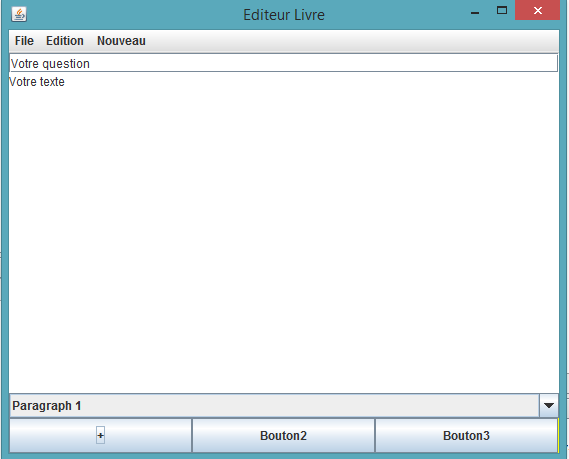
\includegraphics[width=1.1\textwidth]{./images/edit1.png} 
  \end{center}
  \caption{Interface Graphique}
  \label{fig:mon_image}
\end{figure}
\newpage
\paragraph{}Sur la figure 3 on peut voir que : 
\paragraph{} Au niveau du menu \textbf{Nouveau} on a \textbf{ParagrapheTt} qui permet d'ajouter un paragraphe.
\paragraph{}En bas on peut voir le nombre de choix qu'on a fait.
\paragraph{}On peut aussi choisir les paragraphes dans l'ordre qu'on veut. 
 \begin{figure}[ht]
  \begin{center}
    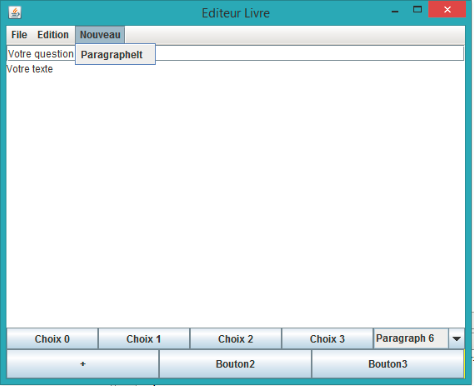
\includegraphics[width=1.1\textwidth]{./images/edit2.png} 
  \end{center}
  \caption{Nouveau Paragraphe}
  \label{fig:mon_image}
\end{figure}
\newpage
\paragraph{}La figure 4 représente les éléments de File et l'ordre de nos choix.
\paragraph{}Sur le menu File on a: Enregistrer, Supprimer, Charger, un bouton + et Quitter.
\paragraph{}Enregister : permet d'enregistrer un fichier.
\paragraph{}Supprimer : permet de supprimer un paragraphe.
\paragraph{}Charger : qui permet de charger un fichier.
\paragraph{}Quitter : qui permet de quitterle jeux.

\begin{figure}[ht]
  \begin{center}
    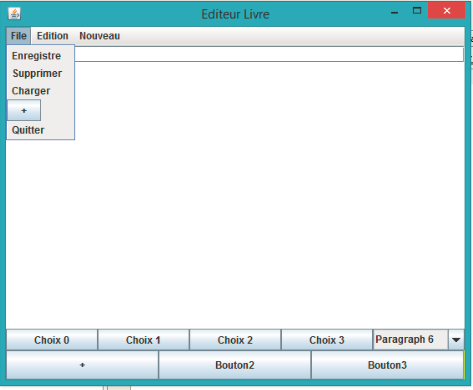
\includegraphics[width=1.1\textwidth]{./images/edit3.png} 
  \end{center}
  \caption{Les éléments du Menu}
  \label{fig:mon_image}
\end{figure}
\newpage
\paragraph{}La figure 5 représente le chargement ou l'enregistrement d'un fichier.
\paragraph{}En cliquant sur Charger on a cette fenêtre qui s'affiche. Ainsi on pourra sélectionner le fichier qu'on veut charger.
\paragraph{}On ferra de la même façon pour enregistrer.
\begin{figure}[ht]
  \begin{center}
    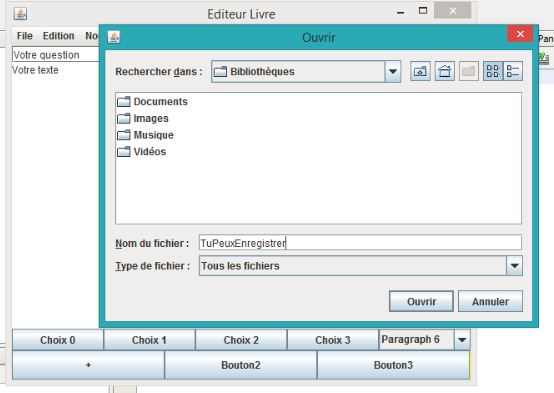
\includegraphics[width=1.1\textwidth]{./images/edit4.png} 
  \end{center}
  \caption{Enregistrement et chargement d'un fichier}
  \label{fig:mon_image}
\end{figure}

\newpage
On a sur la liste déroulante, tous les paragraphes créés. On peut choisir un paragraphe déjà choisi.
\begin{figure}[ht]
  \begin{center}
    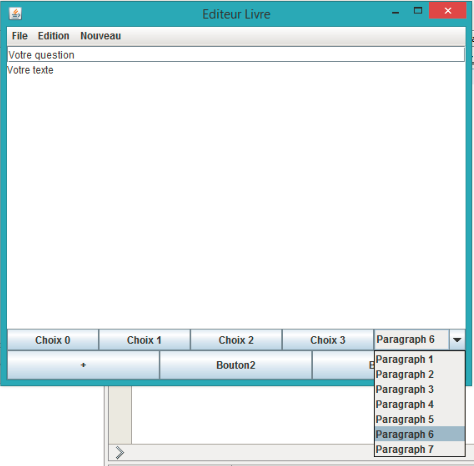
\includegraphics[width=1.0\textwidth]{./images/editF.png} 
  \end{center}
  \caption{ Choix du paragraphe}
  \label{fig:mon_image}
\end{figure}
\newpage


\newpage
\chapter{Conclusion }
    \paragraph{}Au cours de ce rapport, nous avons présenté les différentes étapes « fonctionnement, conception, réalisation » du jeux «  éditeur de livre dont vous êtes le héros ». 
    \\Ce projet a fait l’objet d’une expérience intéressante, meme si nous avions rencontrés quelques difficultés à le réaliser.
    \paragraph{}Malgré tout, nous retiendrons de grandes leçons : l’importance des recherches, la valeur du temps dans la réalisation d’un programme etc.
    \paragraph{}Tout n’est pas parfait certes,mais ce projet nous a permis d’améliorer nos connaissances et nos compétences dans le domaine de la conception logicielle .
\addcontentsline{toc}{part}{Conclusion}
\newpage

%LA BIBLIOGRAPHIE
\newpage
\begin{thebibliography}{9}
\bibitem{ref1} Wikipédia(Livre-Jeu)[ En ligne ]Disponible sur
\href{ https://fr.wikipedia.org/wiki/Livre-jeu#Historique}{https://fr.wikipedia.org/wiki/Livre-jeu#Historique  }
\bibitem{ref2} Wikipédia(Livre-Jeu)[ En ligne ]Disponible sur
\href{ https://fr.wikipedia.org/wiki/Livre-jeu}{https://fr.wikipedia.org/wiki/Livre-jeu  }
\bibitem{ref3} Wikipédia(Livre-Jeu)[ En ligne ]Disponible sur
\href{ https://fr.wikipedia.org/wiki/Livre-jeu#Mecanismes_de_jeu}{https://fr.wikipedia.org/wiki/Livre-jeu#Mecanismes_de_jeu}

\end{thebibliography}

\bibliographystyle{unsrt}%ou plain, abbrv, alpha, apalike, ...

\end{document}
